\section{JEDy: Julia for Evolutionary Dynamics}

The main goal of this project was to kickstart development of a package for Julia for performing the sorts of calculations outlined in the previous section.
My task was to develop the methods for dealing with evolutionary dynamics over finite populations, while my colleague Jesse Duffield developed the methods for infinite populations.
As of writing, we have decent coverage of the methods mentioned in the previous section, and we're able to visualise these results.

The goal for this stage of the package's development was to be able to replicate the results found in a paper by Imhof et. al. \cite{imhofetal} which studied the Prisoner's dilemma.
The heatmap shown in figure \ref{heatmap} is similar (though not as nicely formatted) to the diagram found in Imhof et. al., and displays the same trend found in the paper, namely, that the population spends most of its time in the homogenous TFT state.

\begin{figure}[h]
    \centering
    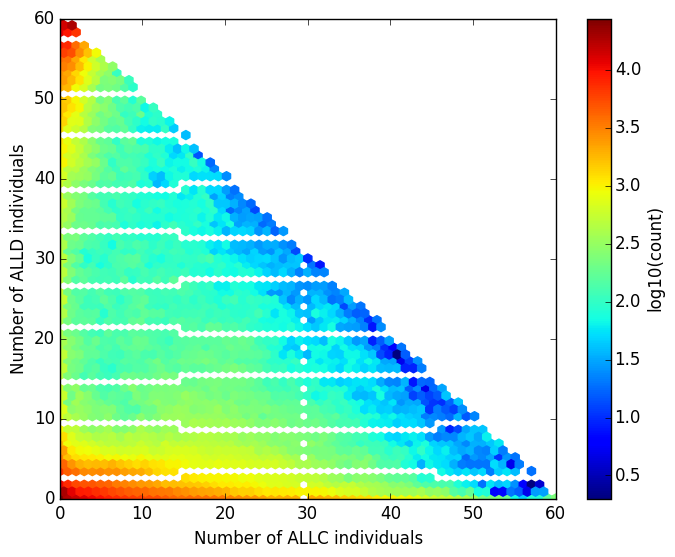
\includegraphics[width = 0.8\textwidth]{graphics/heatmap}
    \caption{A heatmap of state distributions in the iterated prisoners dilemma using a Moran process simulation.
    Parameters are $1 \times 10^6$ iterations at $N = 60, T = 5, R = 3, P = 1, S = 0.1, m = 10, c = 0.8$ with mutation rate $\mu = 1 \times 10^{-2}$ and with linear intensity of selection and intensity of selection 1. The bottom left corner represents the states when the population is mostly TFT. The results here fairly closely match those presented by Imhof et. al. The white lines are artifacts of the plotting process.}
    \label{heatmap}
\end{figure}

We can further confirm that our results match those of Imhof et. al. by studying the plot of the timeseries found in figure \ref{timeseries}.
This plot also shows that the population spends most of its time in the homogenous TFT state.

\begin{figure}[h]
    \centering
    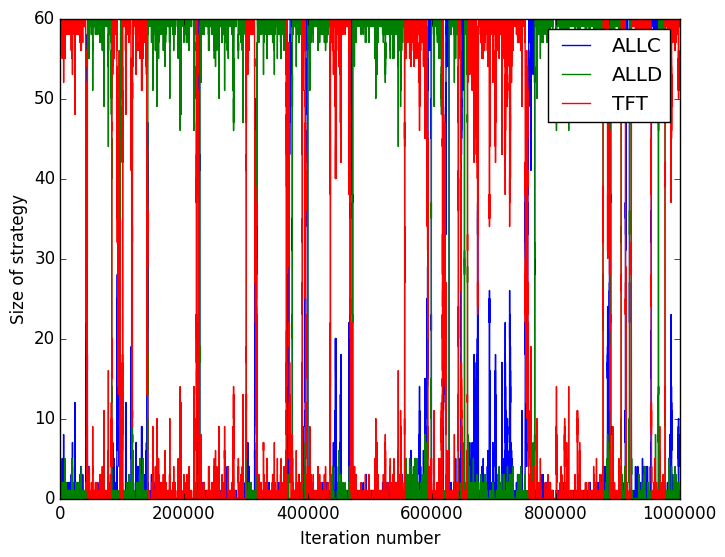
\includegraphics[width = 0.8\textwidth]{graphics/timeseries}
    \caption{A time series of the iterated prisoner's dilemma using a Moran process simulation.
    Parameters are $1 \times 10^6$ iterations at $N = 60, T = 5, R = 3, P = 1, S = 0.1, m = 10, c = 0.8$ with mutation rate $\mu = 1 \times 10^{-3}$ and with linear intensity of selection and intensity of selection 1.
    The population spends most of its time in the TFT state, followed closely by the ALLD state.}
    \label{timeseries}
\end{figure}

Finally, a plot of the intensity of selection against the stationary distribution in figure \ref{stationarydist} shows the expected behaviour.

\begin{figure}[h]
    \centering
    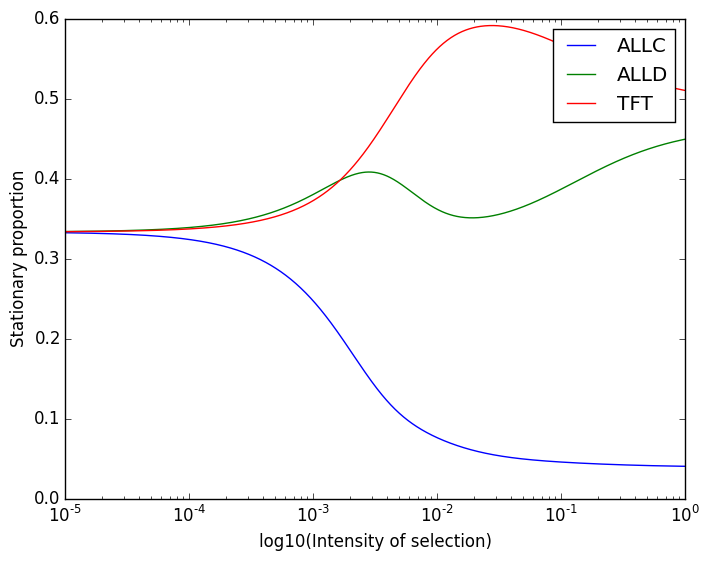
\includegraphics[width = 0.8\textwidth]{graphics/stationarydist}
    \caption{A plot of stationary distribution against intensity of selection for the iterated prisoner's dilemma using a Moran process simulation.
        Parameters are $N = 60, T = 5, R = 3, P = 1, S = 0.1, m = 10, c = 0.8$ with mutation rate $\mu = 1 \times 10^{-3}$ and with linear intensity of selection and intensity of selection between $1 \times 10^{-5}$ and 1 in 1000 setps distributed logarithmically.
        The stationary distribution is evenly distributed among the strategies when intensity of selection is close to zero, as expected.
    When the stationary distribution is close to one, the stationary distribution is dominated by the TFT state, also as expected.}
    \label{stationarydist}
\end{figure}

